% Global Equities Momentum -- replication on free data
%
% Build:  tectonic -X compile paper/gem.tex
% Figures are pulled as vector PDFs from ../output/figures, so the paper always
% shows the exhibits the current code produces. Never edit a figure by hand.

\documentclass[11pt,a4paper]{article}

\usepackage[T1]{fontenc}
\usepackage[utf8]{inputenc}
\usepackage{lmodern}
\usepackage[margin=2.4cm]{geometry}
\usepackage{graphicx}
\usepackage{booktabs}
\usepackage{amsmath}
\usepackage{amssymb}
\usepackage{siunitx}
\usepackage[font=small,labelfont=bf,skip=6pt]{caption}
\usepackage{microtype}
\usepackage{natbib}
\usepackage{xcolor}
\usepackage[hidelinks]{hyperref}

\graphicspath{{../output/figures/}}
\bibliographystyle{apalike}

\sisetup{detect-all, group-separator={,}, table-align-text-after=false}

\setlength{\parskip}{0.45em}
\setlength{\parindent}{0pt}
\renewcommand{\arraystretch}{1.12}

% Figures and tables are read where they appear, so keep them near their text.
\renewcommand{\topfraction}{0.9}
\renewcommand{\textfraction}{0.08}
\renewcommand{\floatpagefraction}{0.8}

\newcommand{\pct}[1]{\SI{#1}{\percent}}

\title{\textbf{Global Equities Momentum on Free Data}\\[0.35em]
       \large A Replication and Extension of Antonacci's Dual Momentum,
       1971--2026}

\author{AUTHOR NAME\thanks{Affiliation. Code and data:
        \url{https://github.com/Petitmarius/Backtest_Strategies}}}

\date{\today}

\begin{document}
\maketitle

\begin{abstract}
\noindent
TODO --- written last, once the results are settled.
\end{abstract}

\vspace{0.5em}
\noindent\textbf{Keywords:} momentum, dual momentum, asset allocation,
market timing, replication.

\section{Introduction}
TODO --- written last.

\section{The Strategy}
\label{sec:strategy}
TODO.

\begin{figure}[htbp]
  \centering
  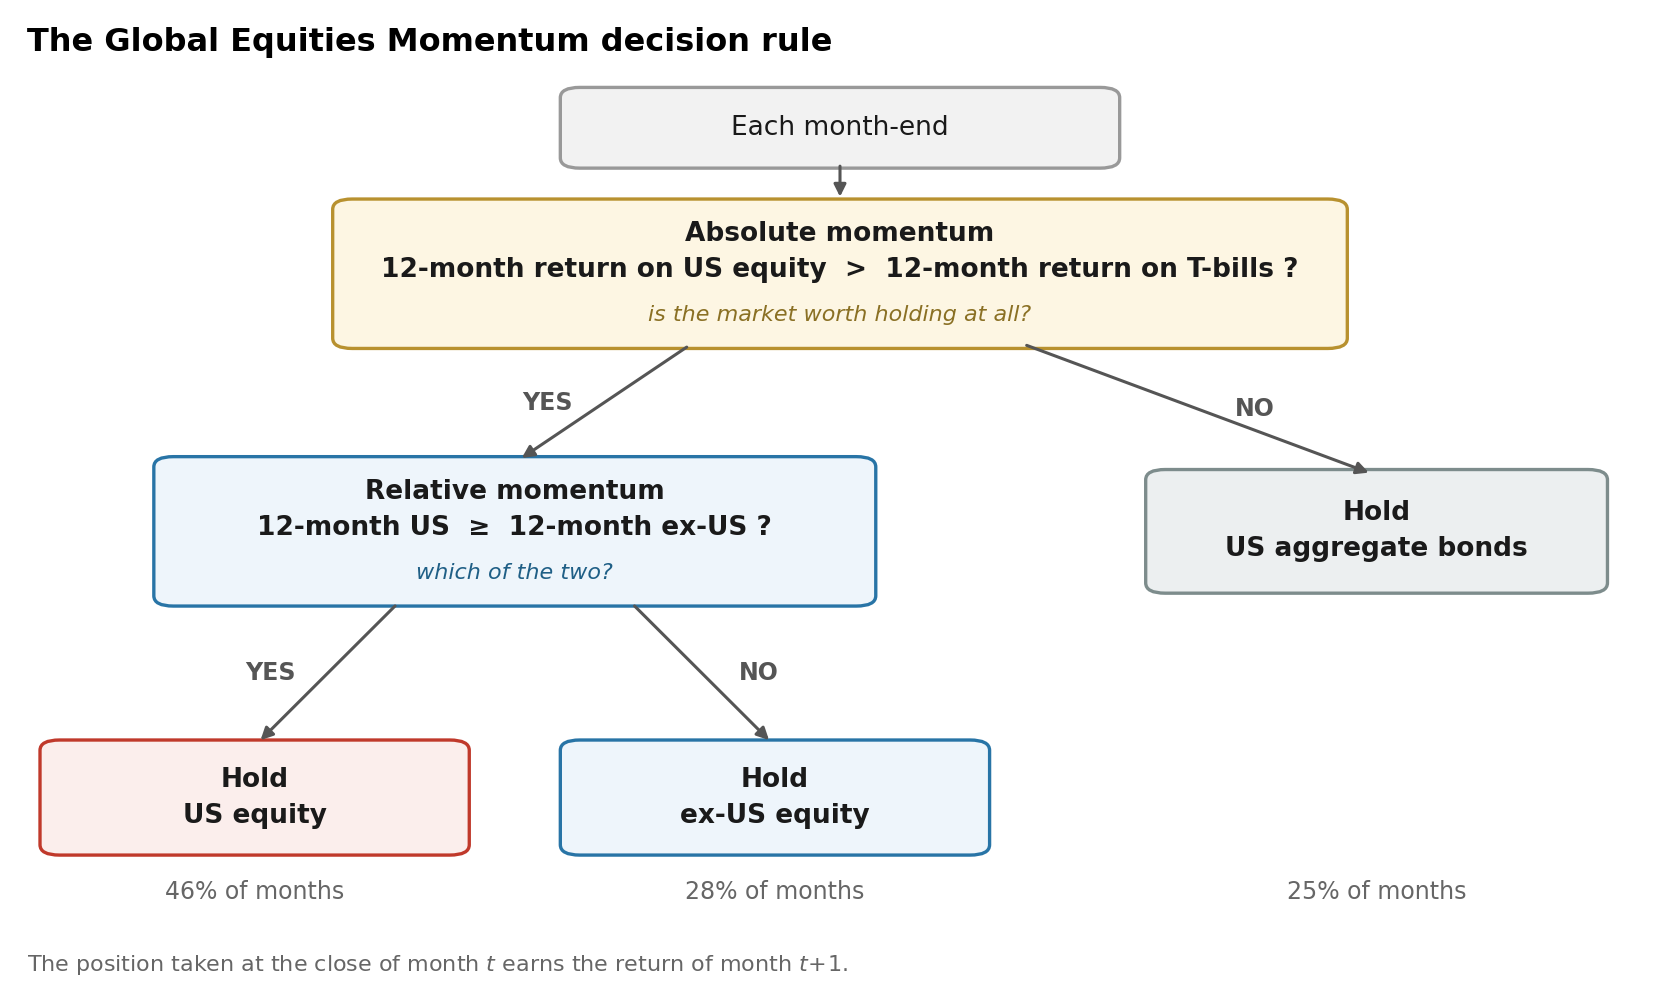
\includegraphics[width=\textwidth]{00_decision_rule.pdf}
  \caption{The Global Equities Momentum decision rule. Absolute momentum
  decides whether to hold equities at all; relative momentum decides which.
  Percentages give the share of months spent in each branch over
  1971--2026.}
  \label{fig:rule}
\end{figure}

\section{Data and Methodology}
\label{sec:data}
TODO.

\begin{figure}[htbp]
  \centering
  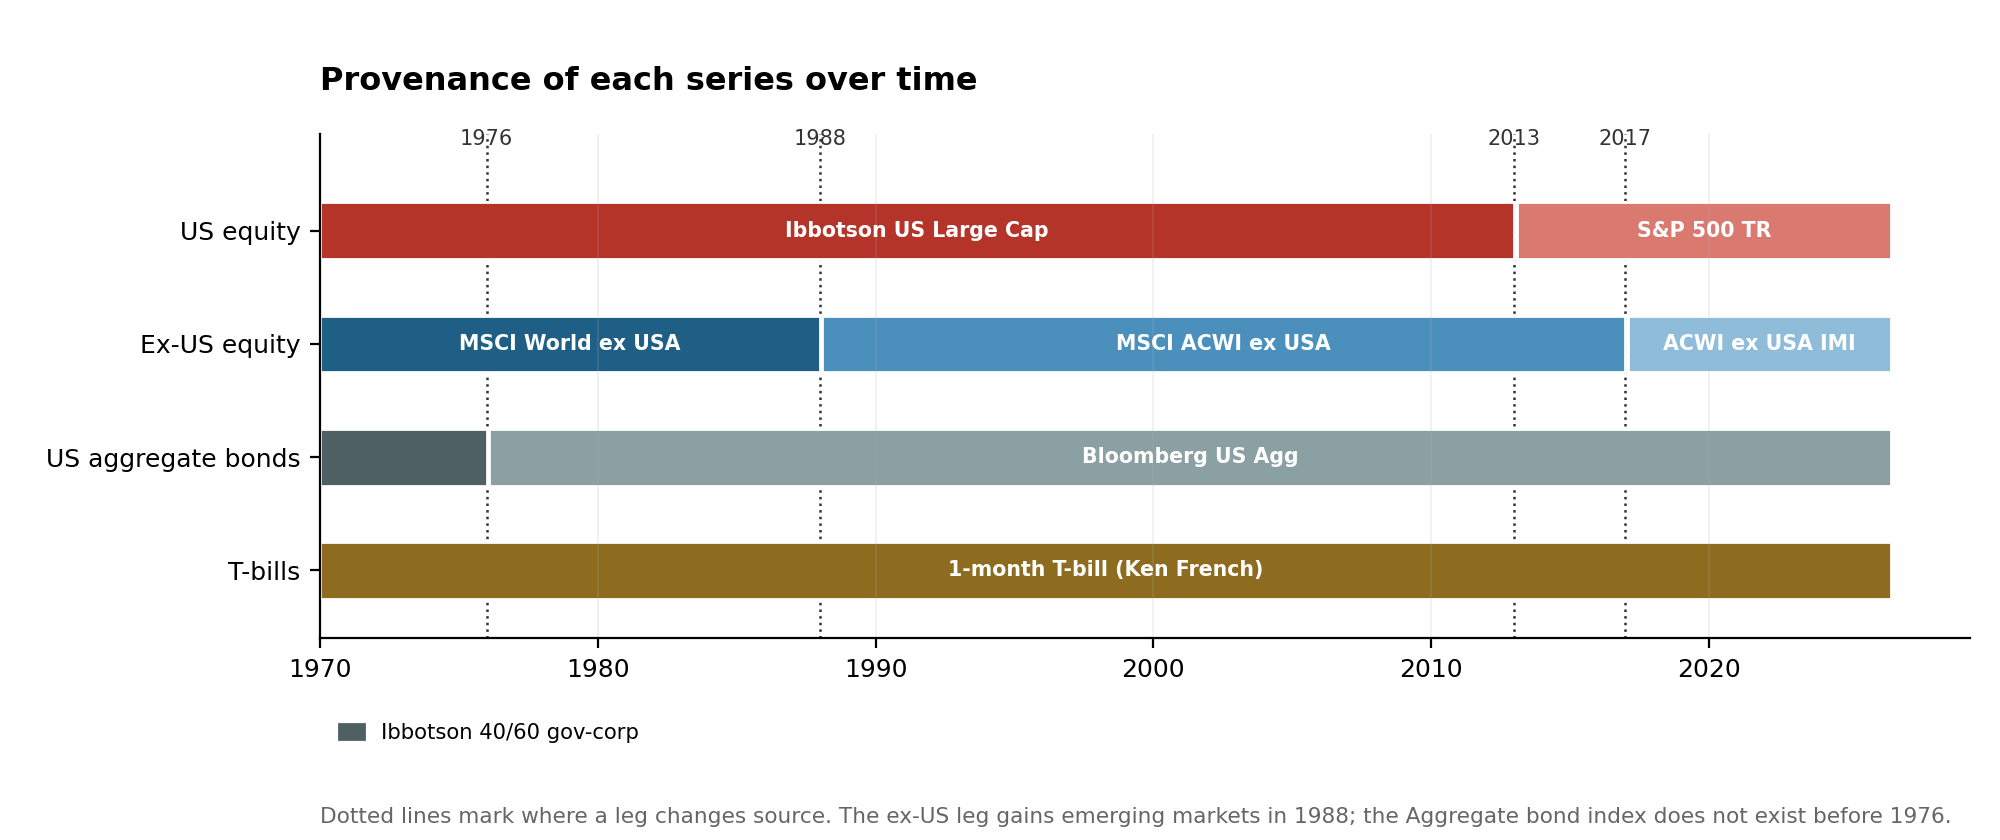
\includegraphics[width=\textwidth]{09_provenance.pdf}
  \caption{Provenance of each series over time.}
  \label{fig:provenance}
\end{figure}

\section{Results}
\label{sec:results}

\subsection{Headline performance}
TODO.

\begin{figure}[htbp]
  \centering
  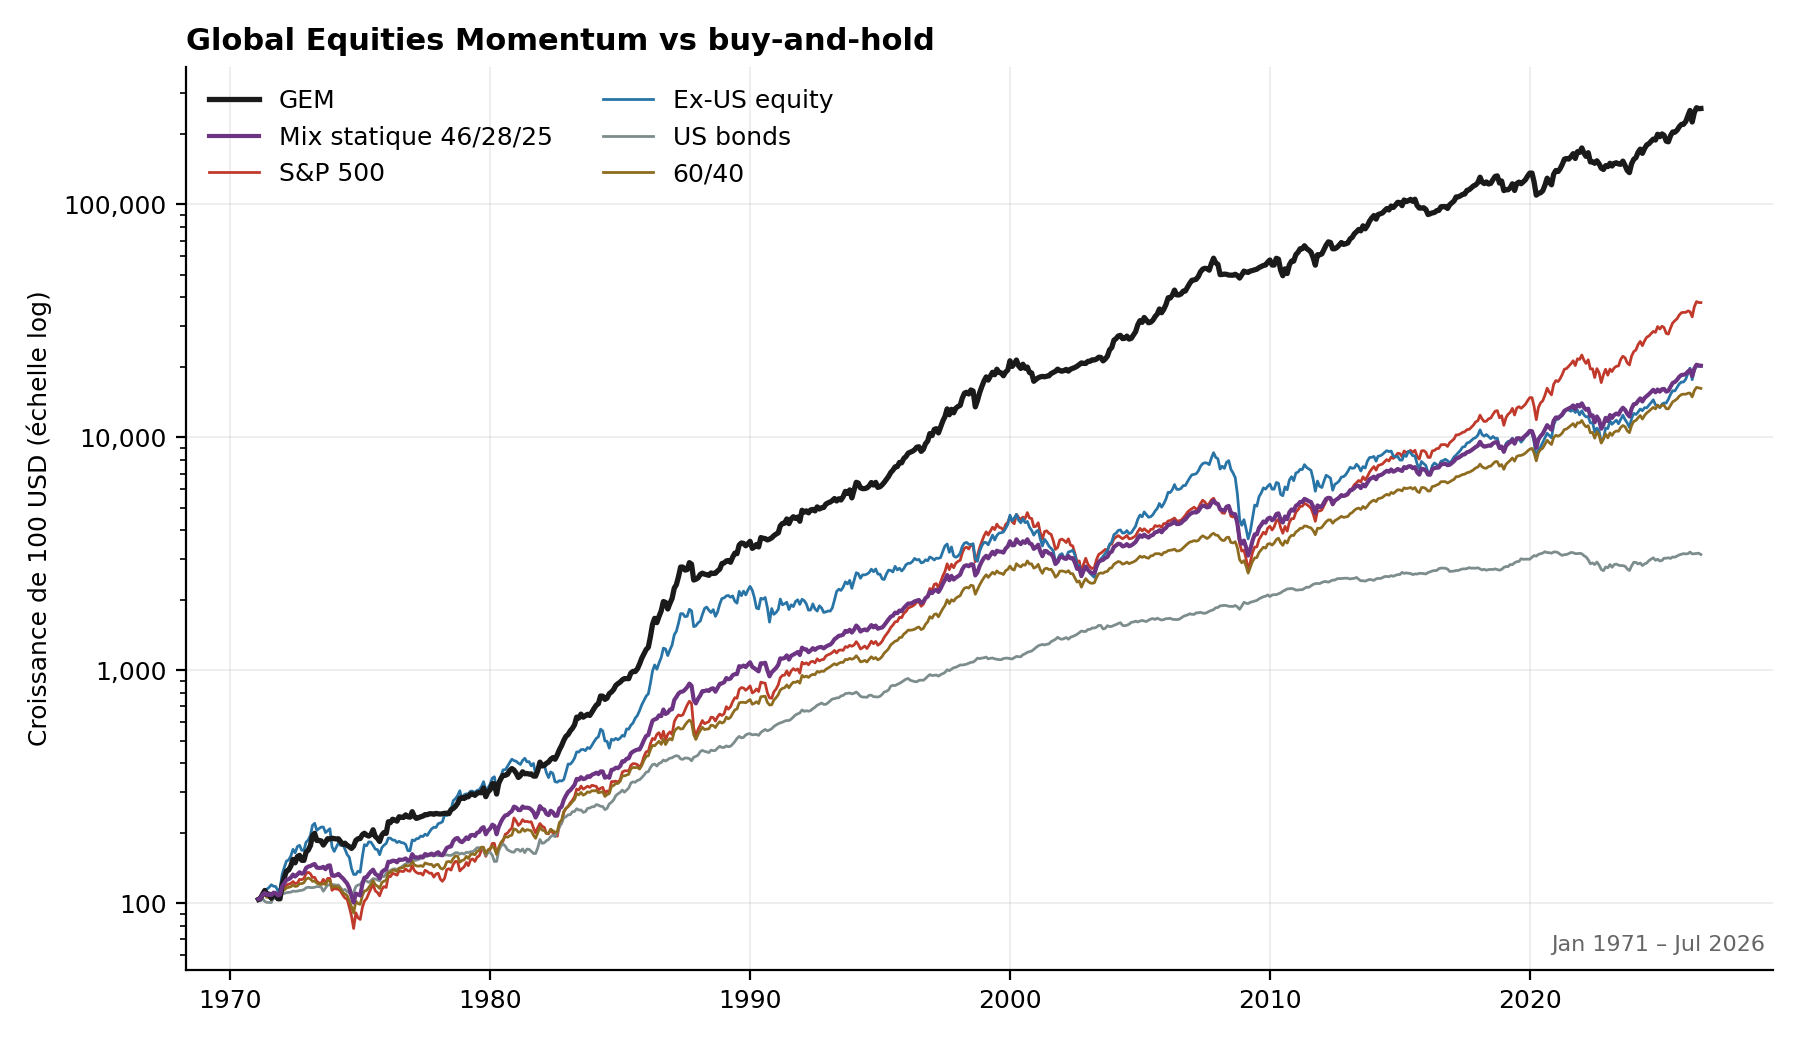
\includegraphics[width=\textwidth]{01_equity_curves.pdf}
  \caption{Growth of \$100, log scale, January 1971 to July 2026.}
  \label{fig:equity}
\end{figure}

\begin{figure}[htbp]
  \centering
  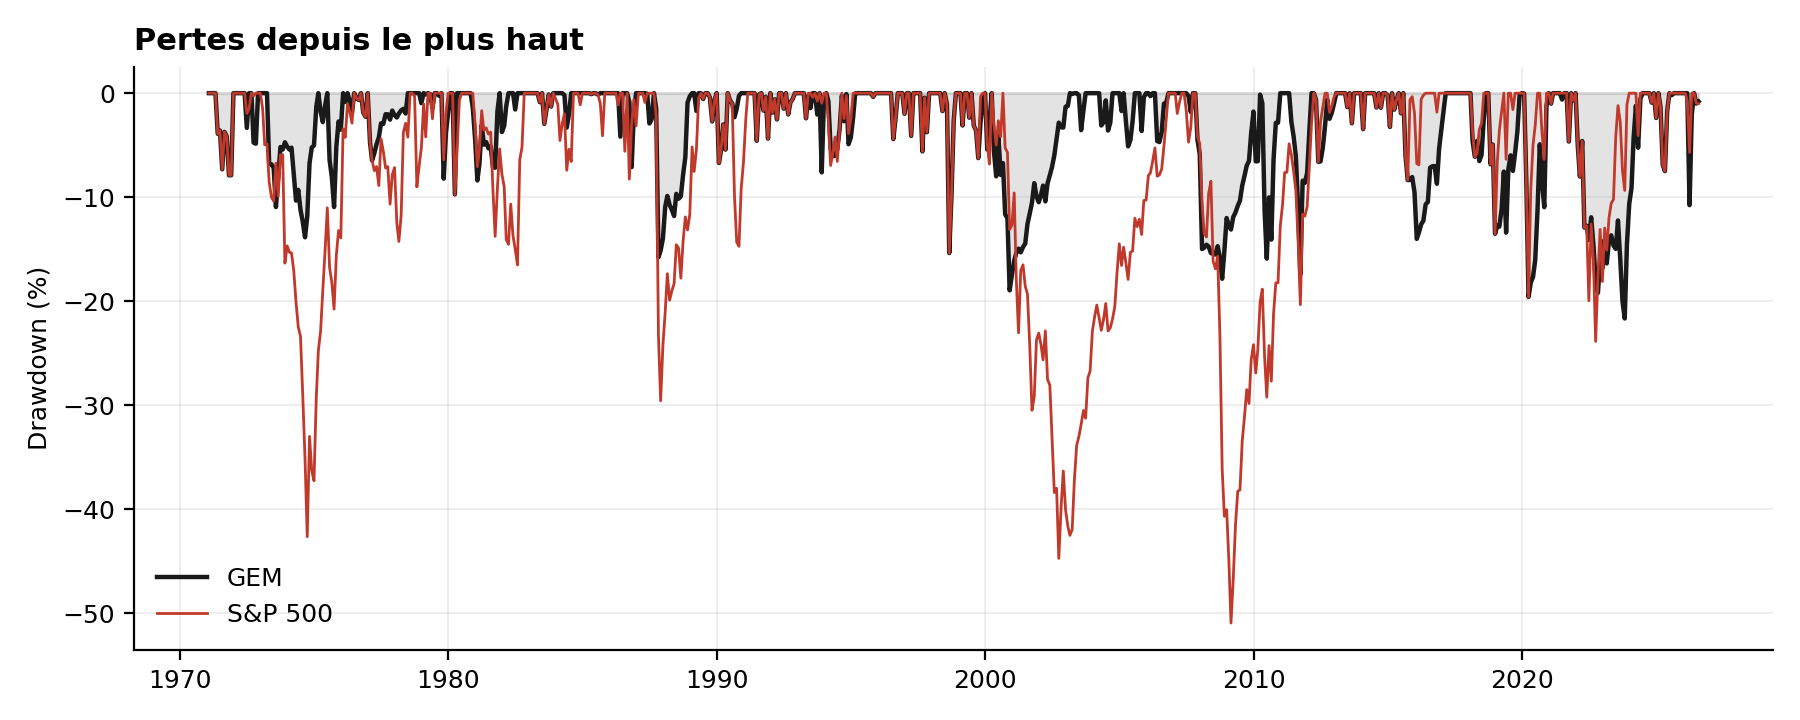
\includegraphics[width=\textwidth]{02_drawdowns.pdf}
  \caption{Drawdowns from prior peak.}
  \label{fig:drawdowns}
\end{figure}

\subsection{Where the return comes from}
TODO.

\subsection{Allocation or timing?}
TODO.

\subsection{Risk-adjusted performance}
TODO.

\subsection{Behaviour through time}
TODO.

\begin{figure}[htbp]
  \centering
  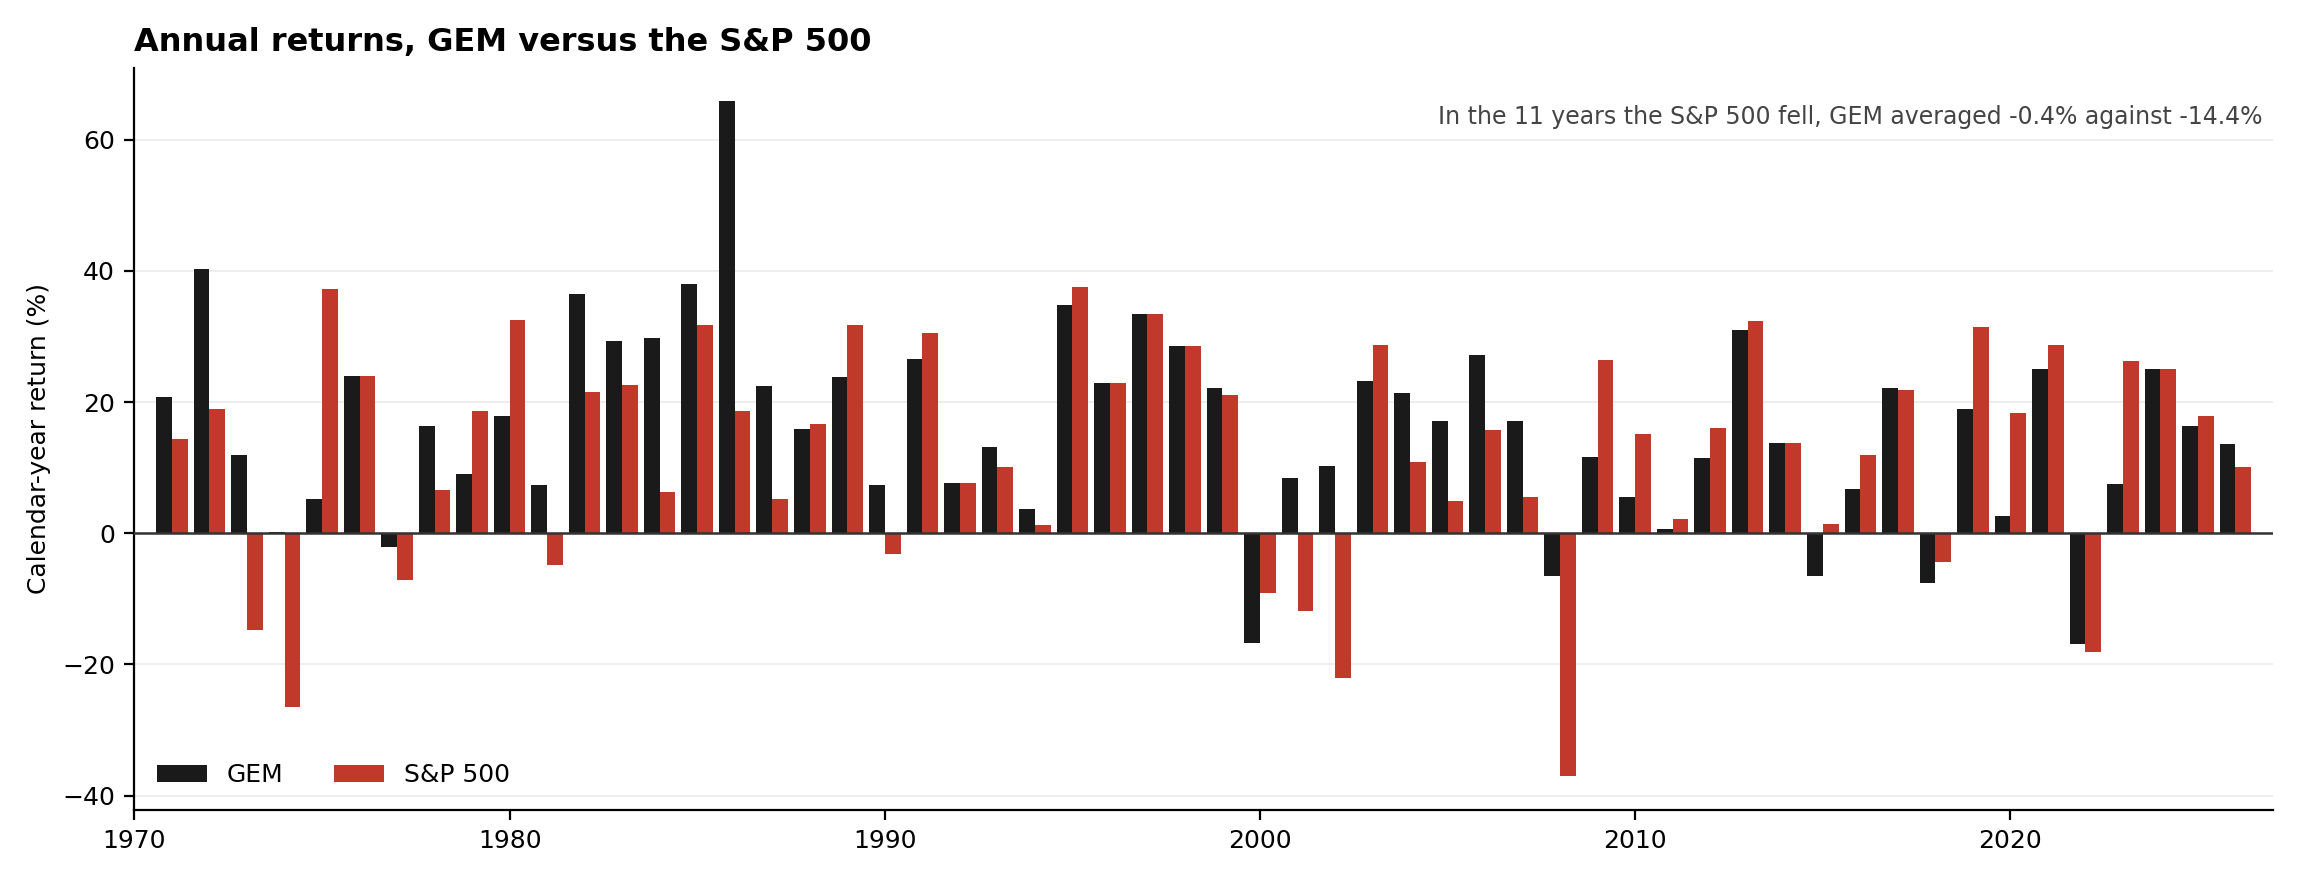
\includegraphics[width=\textwidth]{06_annual_returns.pdf}
  \caption{Calendar-year returns, GEM versus the S\&P 500.}
  \label{fig:annual}
\end{figure}

\begin{figure}[htbp]
  \centering
  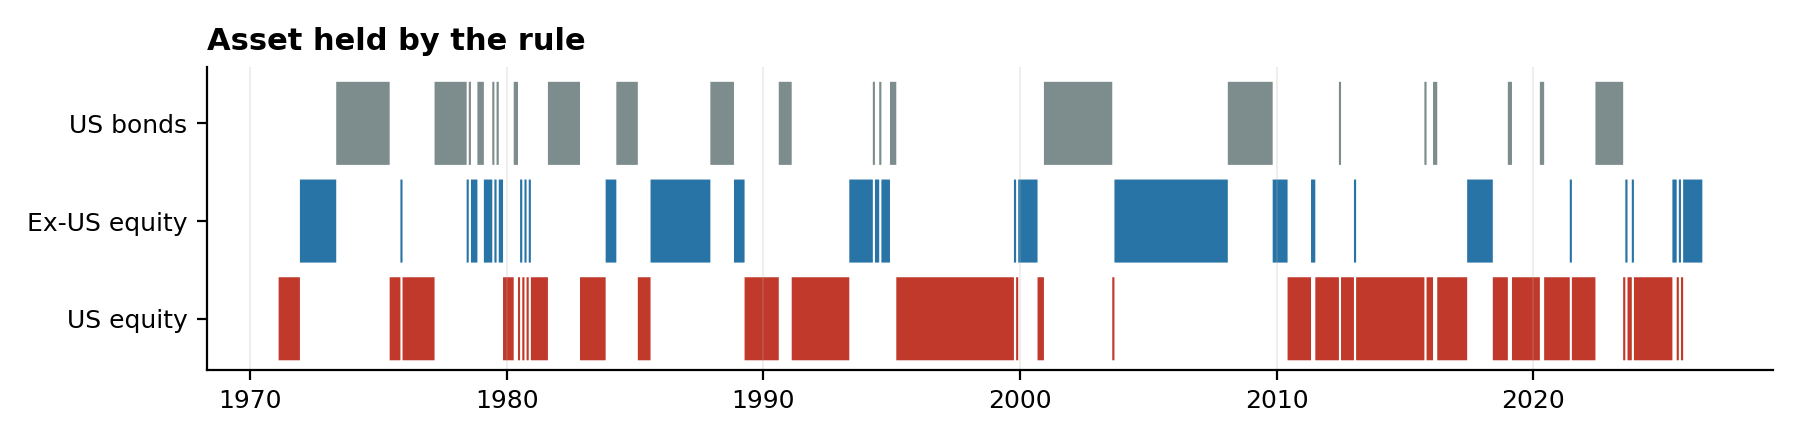
\includegraphics[width=\textwidth]{03_allocation.pdf}
  \caption{Asset held by the rule over time.}
  \label{fig:allocation}
\end{figure}

\begin{figure}[htbp]
  \centering
  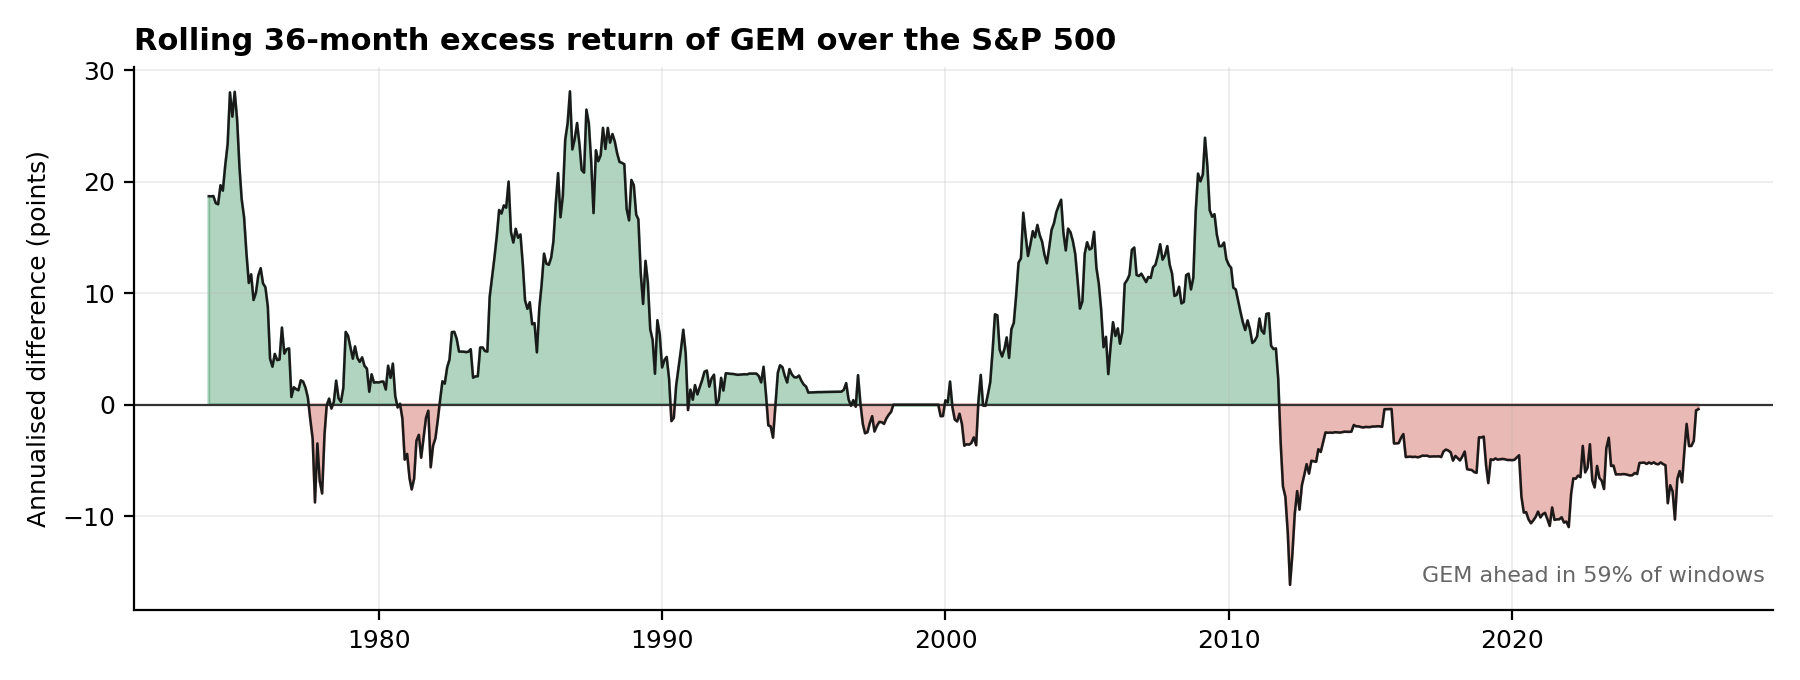
\includegraphics[width=\textwidth]{04_rolling_excess.pdf}
  \caption{Rolling 36-month excess return of GEM over the S\&P 500.}
  \label{fig:rolling}
\end{figure}

\section{Robustness}
\label{sec:robustness}
TODO.

\begin{figure}[htbp]
  \centering
  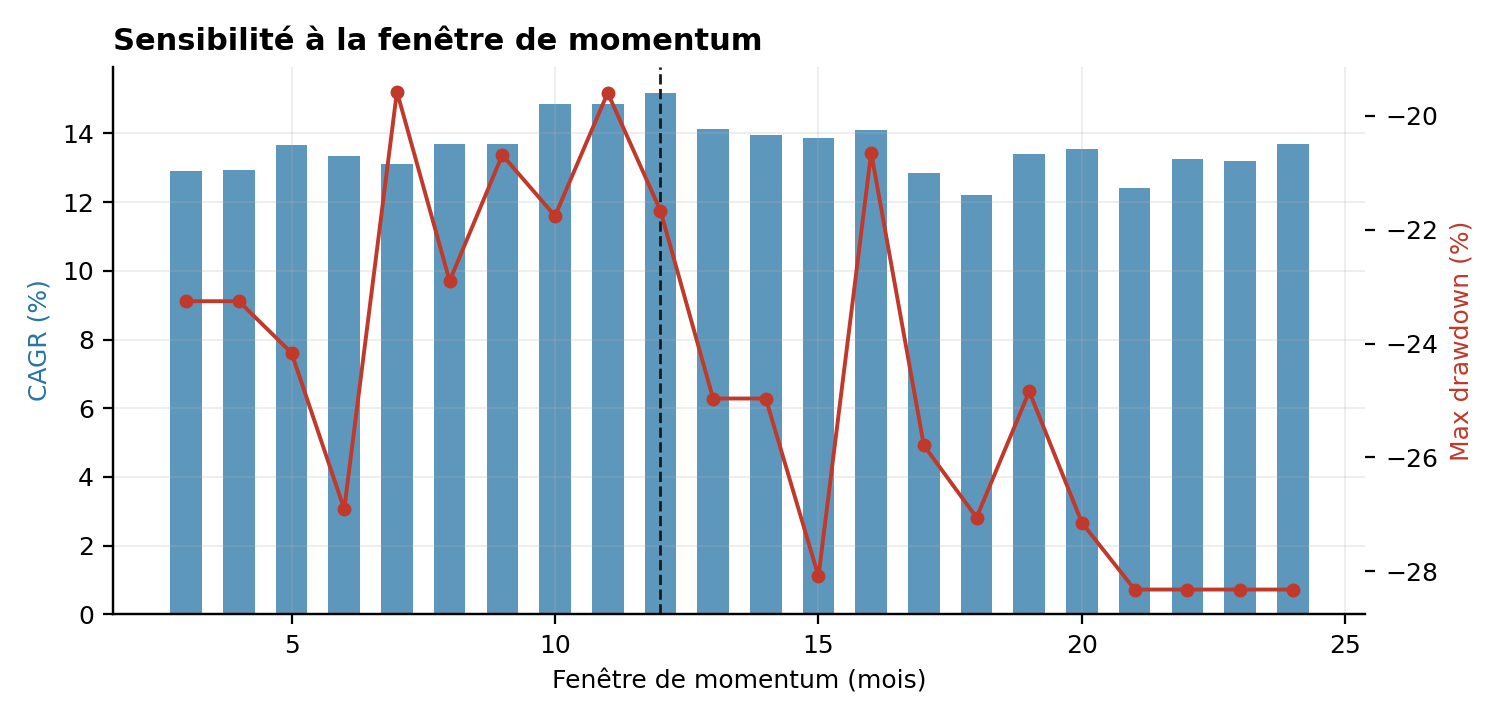
\includegraphics[width=0.86\textwidth]{05_lookback_sensitivity.pdf}
  \caption{Sensitivity to the momentum lookback window.}
  \label{fig:lookback}
\end{figure}

\section{Limitations and Discussion}
\label{sec:limitations}
TODO.

\section{Conclusion}
\label{sec:conclusion}
TODO.

\bibliography{references}

\appendix
\section{Independent Verification of the Dataset}
\label{app:audit}
TODO.

\end{document}
